\documentclass{article}


\usepackage{circuitikz} %Für die Schaltpläne
\usepackage[T1]{fontenc}
\usepackage[utf8]{inputenc}
\usepackage{subcaption}
\usepackage{amsmath}
\usepackage{fancyhdr}
\usepackage{lettrine}
\usepackage{hyperref}
\usepackage{subcaption}
\usepackage{tikz}
\usepackage{cite}
\usepackage{listings}
\usepackage[nottoc, numbib]{tocbibind}
\usepackage{../assets/scripts/tex/color-env}
\usepackage[ngerman]{babel}
%\usepackage{amsmath,amsfonts,stmaryrd,amssymb} % Math packages

\usepackage{enumerate} % Custom item numbers for enumerations

\usepackage[ruled]{algorithm2e} % Algorithms

\usepackage[]{mdframed} % Allows defining custom boxed/framed environments


\mdfdefinestyle{info}{%
	topline=false, bottomline=false,
	leftline=false, rightline=false,
	nobreak,
	singleextra={%
		\fill[black](P-|O)circle[radius=0.4em];
		\node at(P-|O){\color{white}\scriptsize\bf i};
		\draw[very thick](P-|O)++(0,-0.8em)--(O);%--(O-|P);
	}
}

% Define a custom environment for information
\newenvironment{info}[1][Info:]{ % Set the default title to "Info:"
	\medskip
	\begin{mdframed}[style=info]
		\noindent{\textbf{#1}}
}{
	\end{mdframed}
}


\mdfdefinestyle{warning}{
	topline=false, bottomline=false,
	leftline=false, rightline=false,
	nobreak,
	singleextra={%
		\draw(P-|O)++(-0.5em,0)node(tmp1){};
		\draw(P-|O)++(0.5em,0)node(tmp2){};
		\fill[black,rotate around={45:(P-|O)}](tmp1)rectangle(tmp2);
		\node at(P-|O){\color{white}\scriptsize\bf !};
		\draw[very thick](P-|O)++(0,-1em)--(O);%--(O-|P);
	}
}

% Define a custom environment for warning text
\newenvironment{warn}[1][Warning:]{ % Set the default warning to "Warning:"
	\medskip
	\begin{mdframed}[style=warning]
		\noindent{\textbf{#1}}
}{
	\end{mdframed}
}


\usetikzlibrary{shapes}
    \usetikzlibrary{arrows}
    \usetikzlibrary{arrows.meta,topaths}
    \usetikzlibrary{bending}
    \usetikzlibrary{calc}
\title{Elektrotechnik 1 Praktikum 1}


\usepackage[
  includehead,
  headheight = 17mm,
  footskip = \dimexpr\headsep+\ht\strutbox\relax,
  tmargin = 0mm,
  bmargin = \dimexpr17mm+2\ht\strutbox\relax,
]{geometry}

\usepackage{anyfontsize}

\usepackage{xcolor}

\definecolor{DarkGreenBlue}{HTML}{264653}
\definecolor{LightGreenBlue}{HTML}{2A9D8F}
\definecolor{LightOrange}{HTML}{E9C46A}
\definecolor{DarkOrange}{HTML}{F4A261}
\definecolor{RedOrange}{HTML}{E76F51}
\definecolor{BrightRed}{HTML}{D62828}
\definecolor{DeepBlue}{HTML}{003049}

\definecolor{codegreen}{rgb}{0,0.6,0}
\definecolor{codegray}{rgb}{0.5,0.5,0.5}
\definecolor{codepurple}{rgb}{0.58,0,0.82}
\definecolor{backcolour}{rgb}{0.95,0.95,0.92}

\setlength{\parindent}{0pt}

\lstdefinestyle{code}{
    backgroundcolor=\color{backcolour},
    commentstyle=\color{codegreen},
    keywordstyle=\color{magenta},
    numberstyle=\tiny\color{codegray},
    stringstyle=\color{codepurple},
    basicstyle=\ttfamily\footnotesize,
    breakatwhitespace=false,
    breaklines=true,
    captionpos=b,
    keepspaces=true,
    numbers=left,
    numbersep=5pt,
    showspaces=false,
    showstringspaces=false,
    showtabs=false,
    tabsize=2
}

\lstset{style=code}


\pagestyle{fancy}
\fancyhead[L]{\leftmark}
\fancyhead[R]{}
\fancyfoot[L]{}
\fancyfoot[C]{\thepage}
\fancyfoot[R]{
\includegraphics[scale=0.2]{../assets/images/haw.jpg}}
\renewcommand\headrulewidth{0.5pt}


\begin{document}


\thispagestyle{empty}
\begin{tikzpicture}[overlay,remember picture]
  \thispagestyle{empty}
  \fill[black!2] (current page.south west) rectangle (current page.north east);

  \begin{scope}[transform canvas ={rotate around ={45:($(current page.north west)+(-.5,-6)$)}}]

    \shade[rounded corners=18pt, left color=DarkGreenBlue, right color=LightGreenBlue] ($(current page.north west)+(-.5,-6)$) rectangle ++(9,1.5);

  \end{scope}

  \begin{scope}[transform canvas ={rotate around ={45:($(current page.north west)+(.5,-10)$)}}]

    \shade[rounded corners=18pt, left color=LightOrange,right color=DarkOrange] ($(current page.north west)+(0.5,-10)$) rectangle ++(15,1.5);

  \end{scope}

  \begin{scope}[transform canvas ={rotate around ={45:($(current page.north west)+(0.5,-10)$)}}]

    \shade[rounded corners=8pt, right color=DarkOrange, left color=LightOrange] ($(current page.north west)+(1.5,-9.55)$) rectangle ++(7,.6);

  \end{scope}

  \begin{scope}[transform canvas ={rotate around ={45:($(current page.north)+(-1.5,-3)$)}}]

    \shade[rounded corners=12pt, left color=DeepBlue!80, right color=DeepBlue!60] ($(current page.north)+(-1.5,-3)$) rectangle ++(9,0.8);

  \end{scope}

  \begin{scope}[transform canvas ={rotate around ={45:($(current page.north)+(-3,-8)$)}}]

    \shade[rounded corners=28pt, left color=BrightRed, right color=BrightRed!80] ($(current page.north)+(-3,-8)$) rectangle ++(15,1.8);

  \end{scope}

  \begin{scope}[transform canvas ={rotate around ={45:($(current page.north west)+(4,-15.5)$)}}]

    \shade[rounded corners=25pt, left color=RedOrange, right color=DarkOrange] ($(current page.north west)+(4,-15.5)$) rectangle ++(30,1.8);

  \end{scope}

  \begin{scope}[transform canvas ={rotate around ={45:($(current page.north west)+(13,-10)$)}},]

    \shade[rounded corners=22pt, left color=DeepBlue,right color=DarkGreenBlue] ($(current page.north west)+(13,-10)$) rectangle ++(15,1.5);

  \end{scope}

  \begin{scope}[transform canvas ={rotate around ={45:($(current page.north west)+(18,-8)$)}},]

    \shade[rounded corners=8pt, left color=DarkOrange] ($(current page.north west)+(18,-8)$) rectangle ++(15,0.6);

  \end{scope}

  \begin{scope}[transform canvas ={rotate around ={45:($(current page.north west)+(19,-5.65)$)}},]

    \shade[rounded corners=12pt, left color=RedOrange] ($(current page.north west)+(19,-5.65)$) rectangle ++(15,0.8);

  \end{scope}

  \begin{scope}[transform canvas ={rotate around ={45:($(current page.north west)+(20,-9)$)}}]

    \shade[rounded corners=20pt, left color=BrightRed, right color=BrightRed!80] ($(current page.north west)+(20,-9)$) rectangle ++(14,1.2);

  \end{scope}

  \draw[ultra thick,gray] ($(current page.center)+(5,2)$) -- ++(0,-3cm) node[midway,left=0.25cm,text width=5cm,align=right,black!75]{{\fontsize{25}{30} \selectfont \bf GEP\\[10pt] Praktikum 2}} node[midway,right=0.25cm,text width=6cm,align=left,orange]{{\fontsize{70}{86} \selectfont 2021}};

  \node at ($(current page.center)+(0,-4)$) {{\fontsize{40}{72} \selectfont B6-Brücke}};

  \node[text width=8cm,align=center] at ($(current page.center)+(0,-6.5)$) {{\fontsize{16}{20} \selectfont \textcolor{orange}{ \bf 4. Januar}} \\[3pt] Emily Antosch 2519935 \\[3pt] Florian Tietjen \\[3pt] Karl Döring};

\end{tikzpicture}

\newpage


\tableofcontents

\listoffigures

\listoftables


\newpage

\section{Einführung}

Dieser Laborbericht zum dritten Praktikum in Grundlagen der Energietechnik befasst sich  mit den Eigenschaften von Transformatoren im Kontext der Energietechnik. Dabei wird ein Einphasentransformator untersucht und die Parameter des Ersatzschaltbildes ermittelt.\\


\noindent
Im Allgemeinen nutzt man Transformatoren zur Änderung des Spannungspegels von Wechselspannungen. Die Änderung der Spannung von der Primärseite zur Sekundärseite ist dabei direkt proportional zum Übersetzungsverhältnis. Dieses wird durch die Menge an Wicklungen um einen gemeinsamen Eisenkern bestimmt. Dieser zur Verbesserung der Induktion, was zu einem besseren Wirkungsfaktor führt. Über die Eigenschaft von elektrischen Strömen in Leitern Magnetfelder zu erzeugen wird von der Primärseite eine Spannung in der Sekundärseite induziert, welche dem vorher genannten Übersetzungsverhältnis entspricht.\\

\noindent
Um bestimmte physikalische Prozesse, die zu Verlusten bei der Transformation der Spannung entstehen, besser im elektrotechnischen Kontext beschreiben zu können, wird ein allgemeines Ersatzschaltbild verwendet. Dabei beziehen sich die verschiedenen Größen auf die Primärseite. Alle Bauteile mit einer $1$ im Index ist auf der Primärseite, alle Bauteile mit einer $2$ sind hingegen auf der Sekundärseite.

\begin{figure}[h]
  \centering
  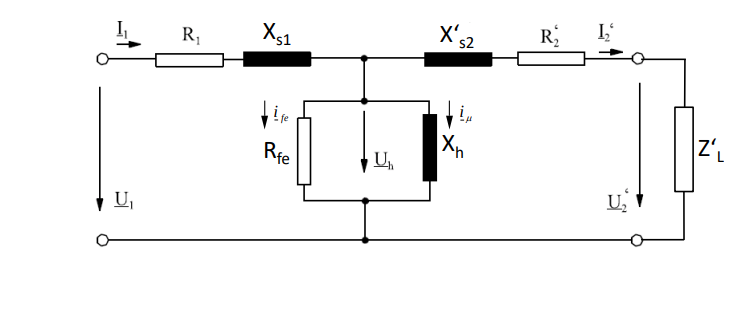
\includegraphics[width=\textwidth]{../assets/images/gep3/esb.png}
  \caption{Ersatzschaltbild eines Transformators}
  \label{fig:esbtrafo}
\end{figure}

\noindent
Die Messungen an unserem Transformator werden maßgeblich von seinen Kenndaten beeinflusst, die wir vom Typenschild im Labor ablesen. Dabei haben wir auf der Primärseite $U_{N} = 380V$ und $I_{N} = 9,5A$ und auf der Sekundärseite $U'_{N} = 220V$ und $I'_{N} = 16A$. Mit diesen Angaben können wir nun bestimmte Messungen die Parameter des ESB Stück für Stück bestimmen.

\newpage
\section{Messung der Wicklungswiderstände beider Seiten}

Wir messen zunächst die Wicklungswiderstände beider Seiten, indem wir ein Ohmmeter an die jeweiligen Klemmen des Transformators anschließen. Die Werte ergeben sich zu:

\begin{equation*}
  \label{eq:1}
  R_{1} = 0,55\Omega, R_{2} = 0,3\Omega
\end{equation*}

\section{Leerlaufversuch am Transformator}

Beim Leerlaufversuch am Transformator wollen wir verschiedene Messungen vornehmen, indem wir auf der Sekundärseite des Transformators keine Last zu schalten, sodass die Klemmen offen sind. Lediglich ein Voltmeter zur Spannungsmessung wird hinzugeschaltet.

\begin{figure}[h]
  \centering
  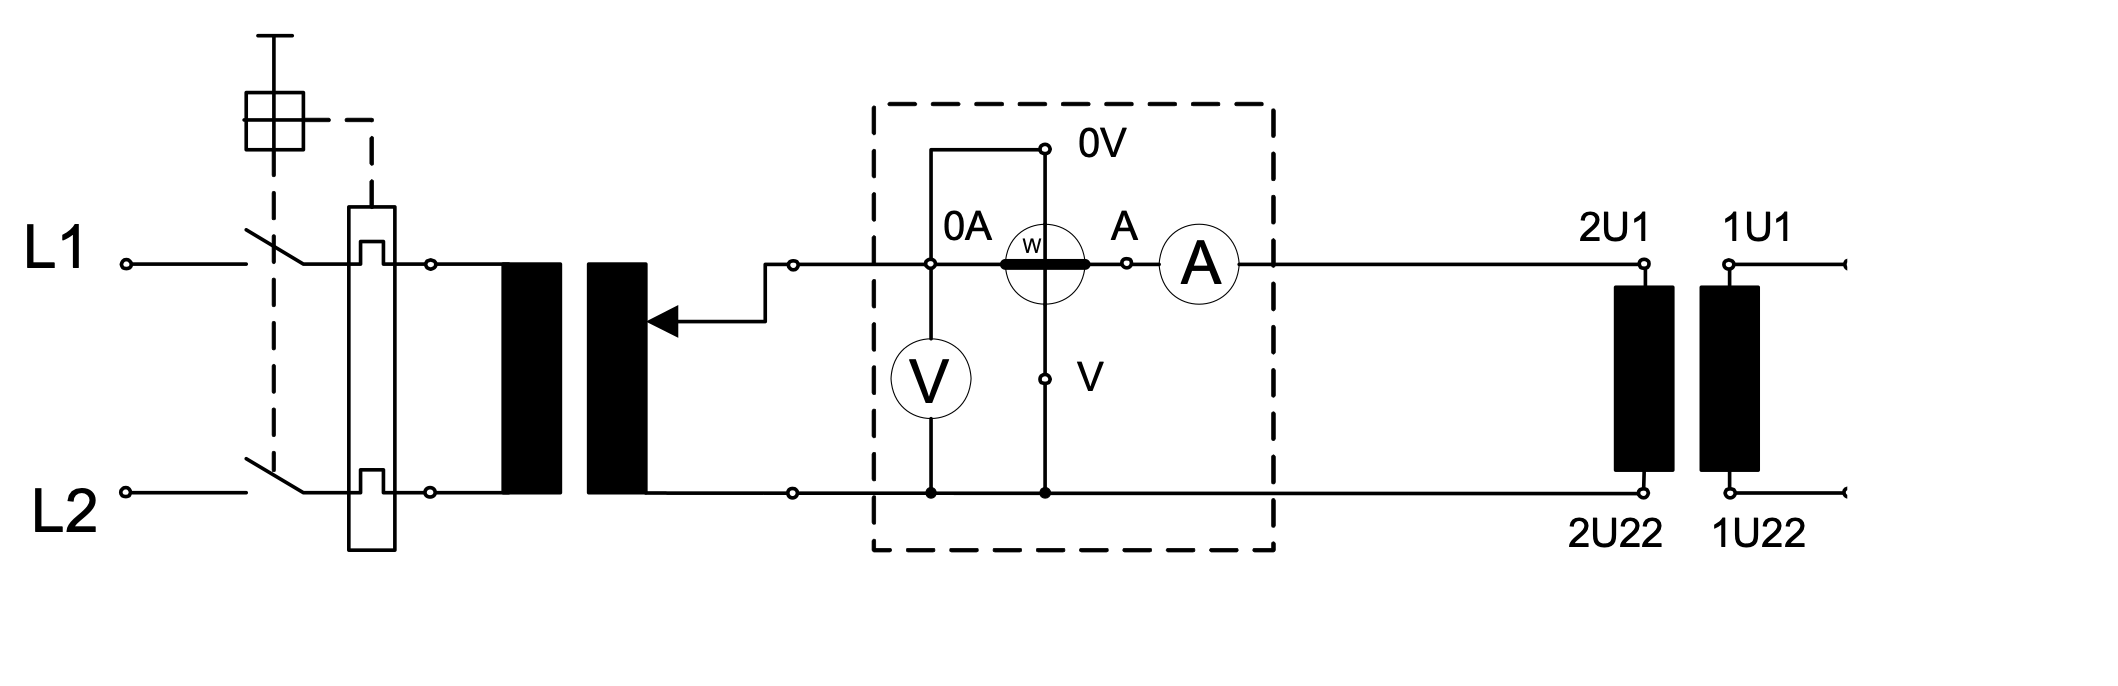
\includegraphics[width=\textwidth]{../assets/images/gep3/leerlauf_aufbau.png}
  \caption{Aufbau des Leerlaufversuchs}
  \label{fig:leerlaufaufbau}
\end{figure}

\subsection{Messung $I_{10}$ und $P_{10}$}
\label{sec:messung-i_10}
\begin{table}[h]
  \centering
  \begin{tabular}{|c|c|c|}
    \hline
    $U_{10}$ & $I_{10}$ & $P_{10}$ \\
    \hline
    $22V$ & $95,4mA$ & $980mW$ \\
    \hline
    $44V$ & $145,6mA$ & $3,56W$ \\
    \hline
    $66V$ & $193mA$ & $7,03A$ \\
    \hline
    $88V$ & $249mA$ & $11,36W$ \\
    \hline
    $110V$ & $323mA$ & $16,86W$ \\
    \hline
    $132V$ & $418mA$ & $22,8W$ \\
    \hline
    $154V$ & $559,8mA$ & $30,15W$\\
    \hline
    $176V$ & $797mA$ & $39,5W$\\
    \hline
    $198V$ & $1,12A$ & $52,02W$\\
    \hline
    $220V$ & $1,61A$ & $71,2W$\\
    \hline
    $242V$ & $2,24A$ & $99,2W$\\
    \hline
  \end{tabular}
  \caption{Strom und Leistung in Abhängigkeit von der Spannung $U_{10}$}
  \label{tab:fifp}
\end{table}

Im Anschluss stellen wir die beiden Werte als Funktion der Spannung $U_{10}$ dar:

\begin{figure}[h]
  \centering
  \begin{subfigure}{.45\textwidth}
    \centering
    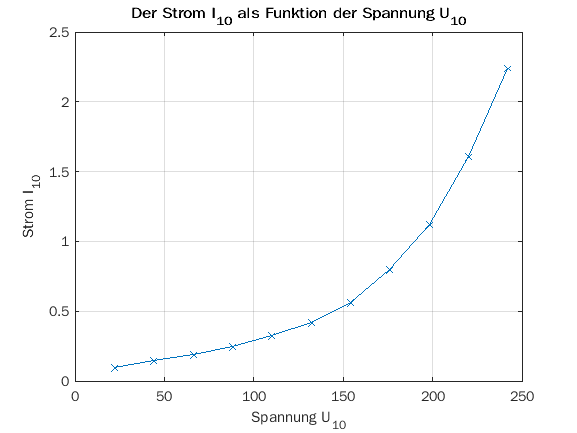
\includegraphics[width=\linewidth]{../assets/images/gep3/u10_i10.png}
    \caption{$I_{10} = f(U_{10})$}
  \end{subfigure}
  \begin{subfigure}{.45\textwidth}
    \centering
    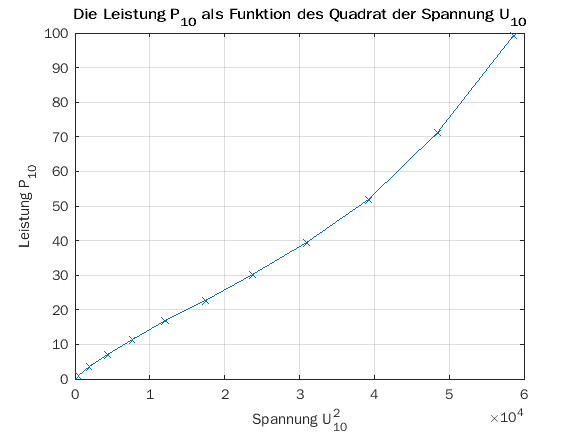
\includegraphics[width=\linewidth]{../assets/images/gep3/u10_p10.png}
    \caption{$P_{10} = f(U_{10}^{2})$}
  \end{subfigure}
  \label{fig:31_242}
  \caption{Die beiden Funktionen $I_{10} = f(U_{10})$ und $P_{10} = f(U_{10}^{2})$}
\end{figure}

\subsection{Bestimmung des Spannungsverhätnisses}
\label{sec:best-des-spann}

Im Nennpunkt für $U_{1N} = 220V$ messen wir beide Seiten des Transformators. Die Primärseite weißt dabei eine Spannung von $U_{2} = 359V$ auf, wodurch man mit

\begin{equation*}
  \textnormal{ü} = \frac{U_{2}}{U_{1N}} = \frac{359V}{220V} = 1.6318
\end{equation*}

einen Spannungsübertragungsverhältnis berechnen. Die Differenz zur theoretischen Übertragung

\begin{equation*}
  \label{eq:3}
  \textnormal{ü} = \frac{U_{2N}}{U_{1N}} = \frac{380V}{220V} = 1.727
\end{equation*}
liegt bei $\Delta \textnormal{ü} = 1.727 - 1.6318 = 0.0952 $, was sich über die Herstellungsdifferenzen der Transformatoren erklären lässt. Gleichzeitig ist zu bemerken, dass der im Labor verwendete Transformator schon relativ alt ist, wodurch möglicherweise bereits Schäden an der Wicklung entstanden sein könnten.


\subsection{Stromverlauf im Nennpunkt}
\label{sec:stromv-im-nennp}

Im nächsten Schritt wird der Stromverlauf bei Nennspannung und bei halber Nennspannung mithilfe einer Stromzange am Oszilloskop betrachtet:

\begin{figure}[h]
  \centering
  \begin{subfigure}{.45\textwidth}
    \centering
    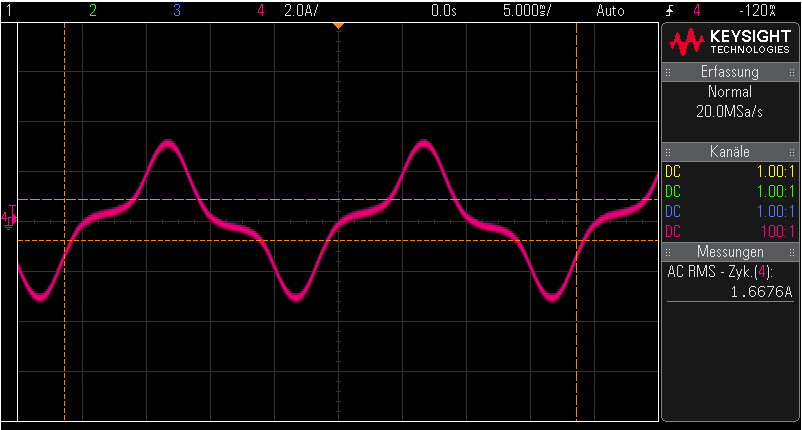
\includegraphics[width=\linewidth]{../assets/images/gep3/trafostrom_voll.png}
    \caption{Volle Nennspannung}
  \end{subfigure}
  \begin{subfigure}{.45\textwidth}
    \centering
    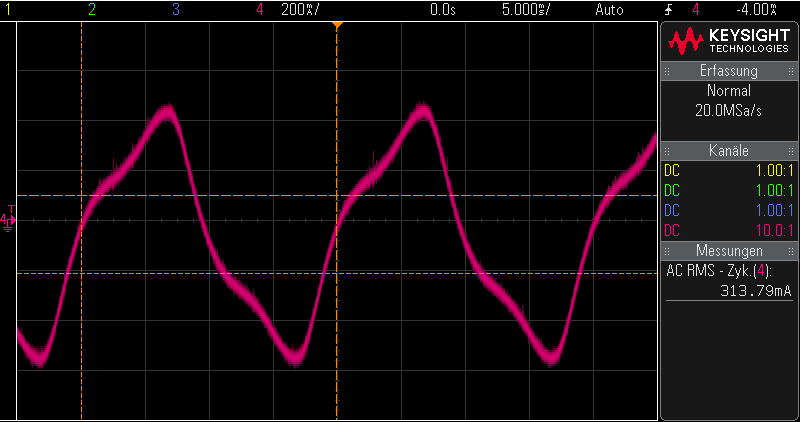
\includegraphics[width=\linewidth]{../assets/images/gep3/trafostrom_halb.png}
    \caption{Halbe Nennspannung}
  \end{subfigure}
  \label{fig:31_242}
  \caption{Der Stromverlauf am Transformator bei voller und halber Nennspannung}
\end{figure}

Es fällt ziemlich deutlich auf, dass bei dem Anlegen der vollen Nennspannung eine vollständige Hystereschleife im Eisenkern des Transformators passiert und der Kern schließlich in die Sättigung geht. Bei halber Nennspannung ist der Effekt auch vorhanden jedoch weitaus weniger deutlich als bei voller Nennspannung. Anhang dieses Beispiels lässt sich die Eigenschaft des Transformators, die sich aus dem Aufbau und Wirkungsweise des Eisenkerns ergibt, gut ableiten. Je nach Umpolung der Magnetfeldkennlinien entsteht eine mehr oder weniger deutliche Hystereschleife im Verlauf des Stroms auf der anderen Seite.

\subsection{Einschaltmoment der Primärseite}
\label{sec:einsch-der-prim}

Mithilfe eines Schaltwinkelstellers betrachtet man nun den Einschaltvorgang auf der Primärseite des Transformators. Dabei können wir unseren Schaltwinkelsteller auf einen bestimmten Winkel, eine Dauer in Perioden und die positive oder negative Halbwelle einstellen.
Bei einer positiven Halbwelle, welche für diese Oszillogramme gewählt wurde, schlägt der Transformator bei voller Umpolung der Magnetfeldkennlinien für die eingestellten Perioden um. Die folgenden drei Bilder sind jeweils für $0^{\circ}$, $45^{\circ}$, $90^{\circ}$ und $50$ Perioden.

\begin{figure}[h]
  \centering
  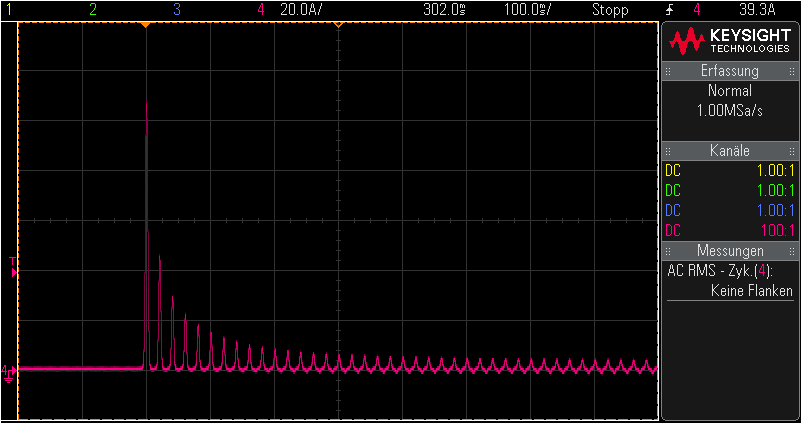
\includegraphics[width=\textwidth]{../assets/images/gep3/einschalt_0deg.PNG}
  \caption{Einschaltverhalten am Transformator bei positiver Halbwelle, $\alpha = 0^\circ$ Zündwinkel und 50 Perioden}
  \label{fig:einschalt_0d}
\end{figure}

Bei einem Einschaltwinkel von $0^{\circ}$ entstehen augenscheinlich die höchsten Einschaltströme. Dies lässt sich dadurch erläutern, dass der Kern nach dem Ausschalten vormagnetisiert ist. Beim Einschalten des Transformators bei der positiven Halbwelle und bei einem Winkel von $0^{\circ}$ wird der Eisenkern zum schlechtesten Zeitpunkt ummagnetisiert, welches die höchste Energie bzw. die höchsten Ströme verursacht. Diesen Effekt nennt man auch Rush-Effekt.

\begin{figure}[h]
  \centering
  \begin{subfigure}{.45\textwidth}
    \centering
    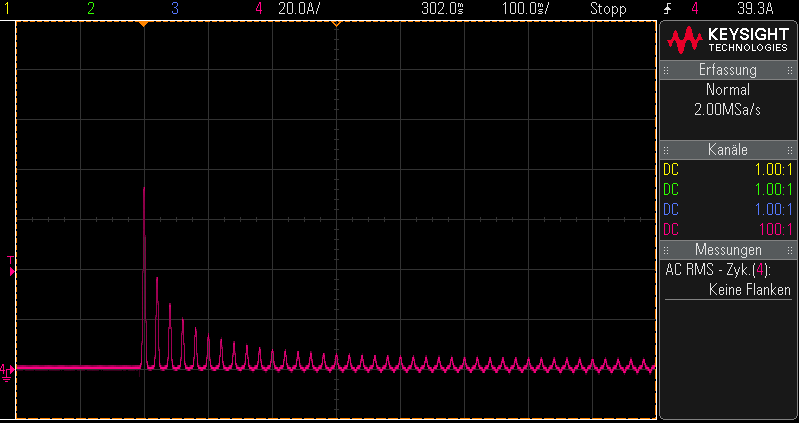
\includegraphics[width=\linewidth]{../assets/images/gep3/einschalt_45deg.png}
    \caption{$\alpha = 45^{\circ}$}
  \end{subfigure}
  \begin{subfigure}{.45\textwidth}
    \centering
    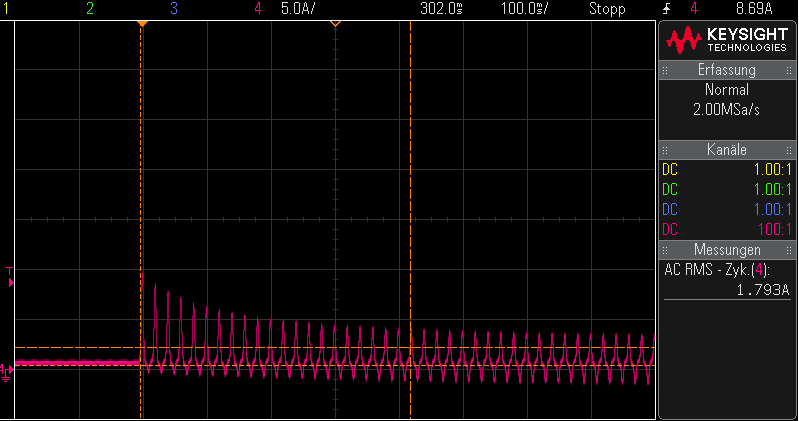
\includegraphics[width=\linewidth]{../assets/images/gep3/einschalt_90deg.png}
    \caption{$\alpha = 90^{\circ}$}
  \end{subfigure}
  \label{fig:31_242}
  \caption{Einschaltverhalten am Transformator bei positiver Halbwelle, $\alpha \in \{45^{\circ}, 90^{\circ}\}$ und 50 Perioden}
\end{figure}

 Bei einem Erhöhen des Winkels verringert sich der Einschaltstrom deutlich. Da durch ein späteres Einschalten in der positiven Halbwelle ein kleiner Effektivwert der Spannung verwendet wird, läuft der Transformator deutlich langsamer und leichter an. Der Rush-Effekt sorgt, ohne Einschaltwinkelsteller, für extrem hohe Einschaltströme die das Netz belasten können. Typischerweise wird daher ein solcher Winkelsteller auf einen Winkel von z.B. $45^{\circ}$ gestellt. Diese Vorkehrung sorgt für geringere Einschaltströme und einen sanften Anlauf, der keine Belastung für das Netz darstellt.

\section{Kurzschlussversuch}
\label{sec:kurzschlussversuch}

Beim Kurzschluss speisen wir nun von der Primärseite vom Stelltransformator ein und schließen die Sekundärseite kurz. Dabei messsen wir dann sowohl $U_{k} = f(I_{k})$ und $P_{k} = f(I_{k})$.

\subsection{Messung der Kurzschlussspannung und der Kurzschlussleistung}
\label{sec:mess-der-kurzschl}

Die Messreihe ergibt folgende Werte:

\begin{table}[h]
  \centering
  \begin{tabular}{|c|c|c|}
    \hline
    $I_{k}$ & $U_{k}$ & $P_{k}$ \\
    \hline
    $11,4A$ & $15,78V$ & $145W$ \\
    \hline
    $10,4A$ & $14,5V$ & $122,7W$ \\
    \hline
    $9,4A$ & $13,1V$ & $98,5W$ \\
    \hline
    $8,4A$ & $11,76V$ & $78,9W$ \\
    \hline
    $7,4A$ & $10,38V$ & $61,52W$\\
    \hline
    $6,4A$ & $8,97V$ & $45,9W$\\
    \hline
    $5,4A$ & $7,58V$ & $37,76W$\\
    \hline
    $4,4A$ & $6,17V$ & $21,73W$\\
    \hline
    $3,4A$ & $4,76V$ & $12,936W$\\
    \hline
    $2,4A$ & $3,4V$ & $7W$ \\
    \hline
    $1,4A$ & $1,9V$ & $2,02W$ \\
    \hline
    $0,4A$ & $0,56V$ & $0,178W$\\
    \hline
  \end{tabular}
  \caption{Messreihe Kurzschlussversuch}
  \label{tab:messkurz}
\end{table}

Im Anschluss tragen wir nun die Spannung $U_{k} = f(I_{k})$ als Funktion des Stromes und die Leistung $P_{k} = f(I_{k}^{2})$ als Funktion des quadrierten Stromes auf:


\begin{figure}[h]
  \centering
  \begin{subfigure}{.45\textwidth}
    \centering
    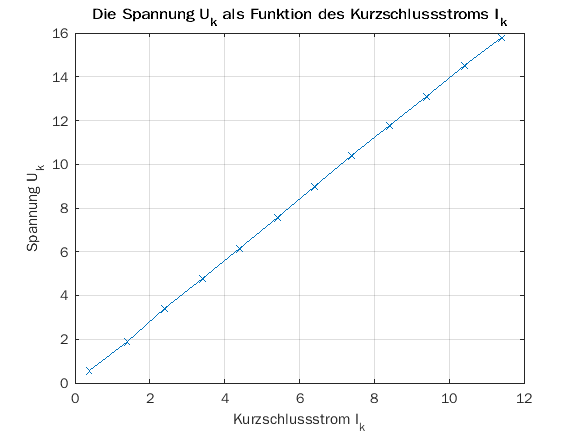
\includegraphics[width=\linewidth]{../assets/images/gep3/ik_uk.png}
    \caption{Oszilloskopbild zur Messung 3.1 für den Winkel $24,2^{\circ}$}
  \end{subfigure}
  \begin{subfigure}{.45\textwidth}
    \centering
    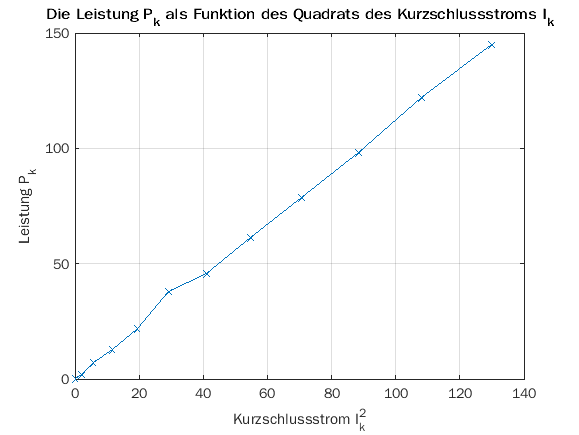
\includegraphics[width=\linewidth]{../assets/images/gep3/ik_pk.png}
    \caption{Oszilloskopbild zur Messung 3.1 für den Winkel $96,2^{\circ}$}
  \end{subfigure}
  \label{fig:31_242}
  \caption{Beispielhafte Bilder vom Oszilloskop}
\end{figure}

\subsection{Bestimmung des Stromübertragungsverhältnisses}

Das Stromübersetzungverhältnis $I_{ü}$ bei $I_{k} \approx I_{n}$ lautet dann

\begin{equation*}
  I_{ü} = \frac{I_{k}}{I'} = \frac{9.4A}{15A} = 0.6266
\end{equation*}

\newpage

\section{Belastungsversuch}
\label{sec:belastungsversuch}

Beim Belastungsversuch verbinden wir mit der Sekundärseite des Transformators ein Potentiometer mit hoher Leistungsbelastbarkeit und messen dann die Spannung $U_{2} = f(I_{2})$ als Funktion des Stromes. Dies machen wir dann für $U_{1} = U_{1n} = konst.$ und $I_{2} \approx 1,2 \cdot I_{n}$.
\begin{figure}[h]
  \centering
  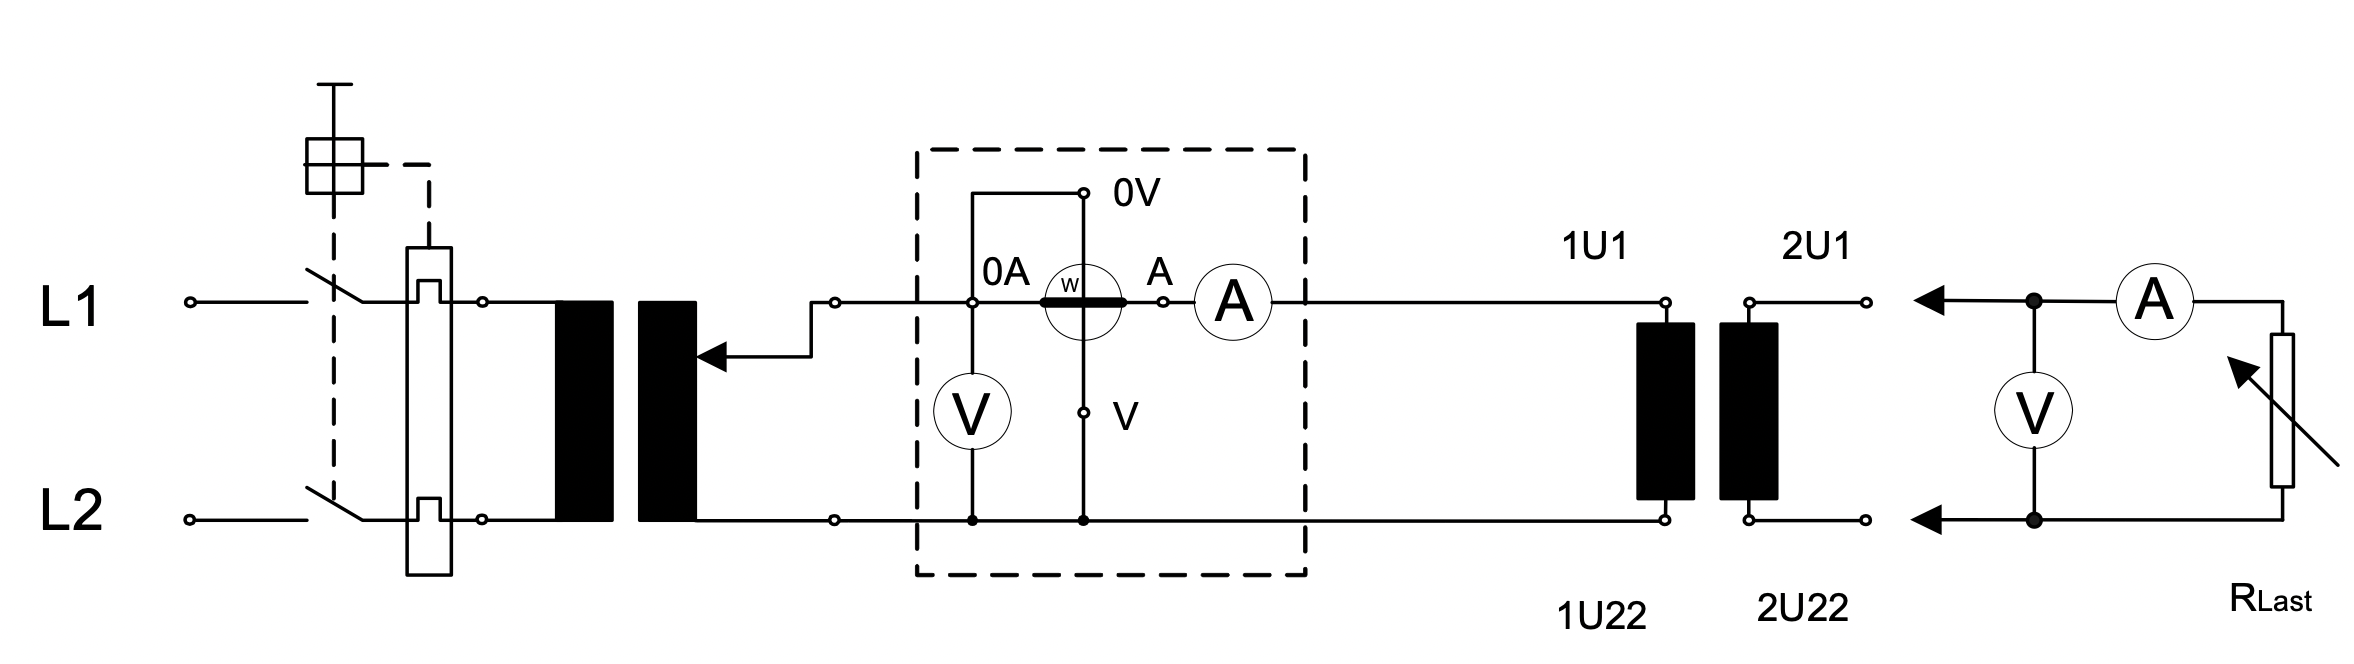
\includegraphics[width=\textwidth]{../assets/images/gep3/belastung_aufbau.png}
  \caption{Aufbau des Belastungsversuchs}
  \label{fig:belastaufbau}
\end{figure}
\subsection{Messung der Spannung, des Stroms und der Leistung mit Wirklast}
\label{sec:messung-der-spannung}


\begin{table}[h]
  \centering
  \begin{tabular}{|c|c|c|c|}
    \hline
    $R_{2}$ & $I_{2}$ & $U_{2}$ & $P_{N}$ \\
    \hline
    $90\Omega$ & $230V$ & $2,55A$ & $688,2W$\\
    \hline
    $78\Omega$ & $232V$ & $2,9A$ & $780W$\\
    \hline
    $66\Omega$ & $231,2V$ & $3,4A$ & $899W$\\
    \hline
    $54\Omega$ & $230V$ & $4,2A$ & $1,08kW$\\
    \hline
    $42\Omega$ & $230V$ & $5,4A$ & $1,33kW$\\
    \hline
    $36\Omega$ & $230V$ & $6,3A$ & $1,56kW$ \\
    \hline
    $30\Omega$ & $230V$ & $7,5A$ & $1,818kW$ \\
    \hline
    $24\Omega$ & $227,4V$ & $9,4A$ & $2,289kW$ \\
    \hline
    $18\Omega$ & $226,6V$ & $12,4A$ & $3,025kW$ \\
    \hline
    $12\Omega$ & $224,1V$ & $18,6A$ & $4,488kW$\\
    \hline
  \end{tabular}
  \caption{Messreihe des Belastungsversuch}
  \label{tab:messbelast}
\end{table}
\newpage
Erneut wird nun die Spannung $U_{2} = f(I_{2})$ als Funktion des Stroms gezeichnet:

\begin{figure}[h]
  \centering
  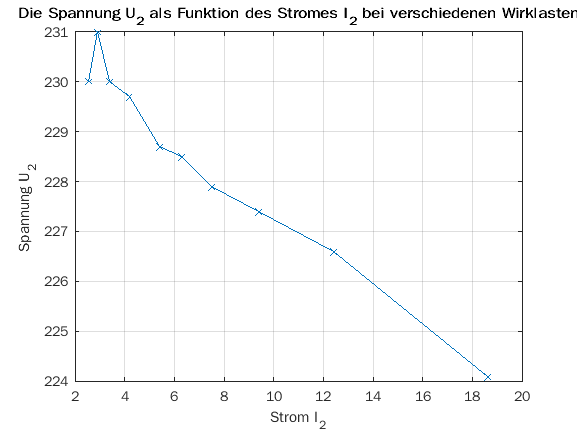
\includegraphics[width=\textwidth]{../assets/images/gep3/i2_u2.png}
  \caption{Die Spannung $U_2 = f(I_2)$ als Funktion des Stromes}
  \label{fig:u2i2}
\end{figure}

\subsection{Messung der Sekundärspannung bei Wirklast}
\label{sec:mess-der-sekund}

\section{Auswertung}
\label{sec:auswertung}

Im Folgenden werden nun die Ergebnisse der Messungen dahingehend ausgewertet, das Modell zur Beschreibung eines Transformators, also das ESB des Einphasentransformators, mit Parametern zu befüllen.


\subsection{Bestimmung der Ersatzimpendanzen $R_{Fe}$ und $X_{1h}$}
\label{sec:best-der-ersatz}

Aus dem Leerlaufversuch können nun die Ersatzimpendanzen $R_{Fe}$ und $X_{1h}$ bestimmt werden. Zunächst wird der Eisenwirkwiderstand $R_{Fe}$ bestimmt. Dieser wird allein von der Wirkleistung erzeugt, daher ergibt sich im Nennpunkt:

\begin{equation*}
  R_{Fe} = \frac{U_{10}^{2}}{P_{10}} = \frac{(220V)^{2}}{71,2W} = 679.775280899\Omega
\end{equation*}

Um nun die die magnetische Hauptreaktanz $X_{1h}$ zu berechnen, betracheten wir das ESB und rechnen dann:

\begin{equation*}
  X_{1h} = \frac{U_{10}}{I_{\mu}} = \frac{U_{10}}{\sqrt{I_{10}^{2}-I_{Fe}^{2}}} = \frac{U_{10}}{\sqrt{I_{10}^{2}-\left(\frac{U_{1N}}{R_{Fe}}\right)^{2}}} = \frac{220V}{\sqrt{1.61A^{2}-0.323638A^{2}}} = \frac{220V}{1.5771A} = 139,5\Omega
\end{equation*}

\subsection{Bestimmung der Ersatzimpedanzen $R_{k}$ und $X_{k}$}
\label{sec:best-der-ersatz-1}

Aus dem Kurzschlussversuch können nun im Anschluss die beiden Impendanzen $R_{k}$ und $X_{k}$ bestimmt werden. Zunächst wird der Kurzschlusswiderstand $R_{k}$ im Nennbetrieb bestimmt über:

\begin{equation*}
  R_{k} = \frac{P_{k}}{I_{k}^{2}} = \frac{98,5W}{(9,4A)^{2}} = 1.11\Omega
\end{equation*}

Als nächstes können wir nun auch die Kurzschlussreaktanz über

\begin{equation*}
  X_{k} = \sqrt{Z_{k}^{2}-R_{k}^{2}} = \sqrt{\left(\frac{U_{k}}{I_{k}}\right)^{2}-R_{k}^{2}} = \sqrt{\left(\frac{13.1V}{9.4A}\right)^{2} - (1.11\Omega)^{2}} = 0.8426\Omega
\end{equation*}

berechnen.

Um nun $R_{k}$ mit dem in Messreihe 2 ermittelten Wicklungswiderständen zu vergleichen, transformieren wir $R_{2}$ auf die Primärseite über:
\[
  R_{2}' = R_{2}\cdot \textnormal{ü}^{2} = 0.3\Omega \cdot 1,6318^{2} = 0.7988\Omega
\]

und rechnen dann:

\[
  R_{k} = R_{1} + R_{2}' = 0,55 + 0,7988 = 1.3488
\]

Die Abweichung des gemessenen $R_{k}$ und des aus der Wicklungswiderstandsmessung ermittelten $R_{k}$ beträgt ca. $23\%$, was ziemlich beachtlich ist. Diese Abweichung lässt sich größtenteils auf Messungenauigkeiten und der Ungenauigkeit des Ohmmeters bei kleinen Messbereichen.


\subsection{Ermittlung des Wirkungsgrads für den Nennpunkt}
\label{sec:ermittl-des-wirk}

Zuletzt wollen wir nun den Wirkungsgrad mit verschiedenen Methoden bestimmen. Dabei nutzen wir sowohl den Belastungsversuch als auch die Ergebnisse der verschiedenen Versuche, um ein Ergebnis zu berechnen. Wir bestimmen den Wirkungsgrad nun zunächst über direkte Messung:

\begin{equation*}
  \eta_{mess} = \frac{P_{ab}}{P_{zu}} = \frac{U_{2} \cdot I_{2}}{P_{1}} = \frac{224,1V \cdot 18.6A}{4,488kW} = 0,9286 \implies 92,68\%
\end{equation*}

Zum Vergleich berechnen wir den Wirkungsgrad über die Ergebnisse der anderen Versuche:

\begin{equation*}
  \eta_{rech} = \frac{P_{ab}}{P_{zu}} = \frac{P_{1} - P_{10} - P_{k}}{P_{1}} = \frac{4,488kW - 98,5W - 71,2W}{4,488kW} = 0,9621 \implies 96,21\%
\end{equation*}

Wir erkennen eine Abweichung von ca. $\Delta \eta = \eta_{rech} - \eta_{mess} = 0,9621 - 0,9286 = 0.335$, also $3,35\%$. Dies lässt sich anhand von Messungenauigkeiten und auch Ungenauigkeiten in den Messgeräten erklären, die über die verschiedenen Versuche zum Einsatz kamen. Im Anschluss bestimmen wir nun auch den Wirkungsgrad bei einer Temperatur von $75^{\circ}C$ bestimmen.

Mithilfe des vorher bestimmten Werte $R_{k,20^{\circ}C} = 1,11\Omega$ und dem Temperaturkoeffizienten von Kuper $\alpha_{Cu} = 3,93 \cdot 10^{-3}K^{-1}$ können wir nun den Widerstandswert bei $75^{\circ}C$ berechen:

\begin{equation*}
  \label{eq:4}
  R_{k,75^{\circ}C} = R_{k, 20^{\circ}C} \cdot (1+\alpha_{Cu}\Delta\vartheta) = 1,11\Omega \cdot (1+3,93\cdot 10^{-3}K^{-1}\cdot 55K) = 1,3499\Omega
\end{equation*}

Nun wollen wir noch den Leistungsverlust für diese Erhöhung der Last berechnen:

\begin{equation*}
  \label{eq:2}
  \Delta P_{k} = I_{k}^{2} \cdot (R_{k,75^{\circ}C} - R_{k,20^{\circ}C}) = 9.4^{2}A^{2} \cdot 0,2399\Omega = 21,197W
\end{equation*}

Damit können wir nun unseren angepassten Wirkungsgrad von

\begin{equation*}
  \label{eq:5}
  \eta = \frac{P_{N} - P_{10} - P_{k} - \Delta P_{k}}{P_{N}} = \frac{4488W-71,2W-98,5W-21,197W}{4488W} = 0,957 \implies 95,7\%
\end{equation*}
Der Wirkungsgrad ist also, wie erwartet, geringer als der theoretische Wirkungsgrad ohne Berücksichtigung der Temperatur, da dadurch noch mehr Widerstand in den Spulen beim Übertragen der Energie entsteht.

\section{Konklusion}
\label{sec:konklusion}

Wir haben in diesem Praktikum sehr viele Eigenschaften des Einphasentransformators verinnerlichen können. Auch das Berechnen der wichtigen Eckdaten des Ersatzschaltbildes des Transformators konnte geübt werden. Das strukturierte Messen von Transformatoren wurde durchgeführt, weshalb man nun die Eigenarten bekannt sind. Auch das Nutzen von verschiedenen Analysemöglickeiten wie zum Beispiel das graphische Darstellen von Messdaten stellte sich als sehr sinnvoll heraus. Besonders interessant war das Verwenden des Stellwinkelstellers zur genauen Untersuchung des Einschaltverhaltens des Transformators.

\end{document}
